\documentclass[12pt, a4paper, openany]{report}
\def\VersionRapport{1.0}
\usepackage[utf8]{inputenc} % un package
\usepackage[T1]{fontenc}      % un second package
\usepackage[francais]{babel}  % un troisième package
\usepackage{layout}
\usepackage[top=2.7cm, bottom=2.5cm, left=3.5cm, right=3cm]{geometry}
\usepackage{setspace}
\frenchbsetup{StandardLists=true} % à inclure si on utilise \usepackage[french]{babel}
%\usepackage{enumitem}
\usepackage[shortlabels]{enumitem}
\usepackage{amssymb}
\usepackage{color}
\usepackage{listings}
\definecolor{dkgreen}{rgb}{0,0.6,0}
\definecolor{gray}{rgb}{0.5,0.5,0.5}
\definecolor{mauve}{rgb}{0.58,0,0.82}
\definecolor{rougecerise}{rgb}{0.73,0.043,0.043}
\lstset{frame=tb,
  language=Matlab,
  aboveskip=3mm,
  belowskip=3mm,
  showstringspaces=false,
  columns=flexible,
  basicstyle={\small\ttfamily},
  keywordstyle=\color{blue},
  commentstyle=\color{dkgreen},
  stringstyle=\color{mauve},
  breaklines=true,
  breakatwhitespace=true,
  tabsize=3,
  breaklines=true,
  morekeywords={matlab2tikz},
  morekeywords=[2]{1}, 
  keywordstyle=[2]{\color{black}},
  identifierstyle=\color{black},
  numbers=left,
  numberstyle={\tiny \color{black}},
  numbersep=9pt, 
  emph=[1]{for,end,break},
  emphstyle=[1]\color{red}
}
\usepackage{multirow} % pour les tableaux
\usepackage[table]{xcolor} % pour les tableaux
\usepackage{verbatim}
%\usepackage{subcaption}
\usepackage{graphicx}
\usepackage{moreverb}
\usepackage{url}
\usepackage{pst-all}
\usepackage{eso-pic,graphicx}
\usepackage{caption} 
\usepackage[colorlinks=true,urlcolor=blue,linkcolor=red]{hyperref}
\usepackage{array}
\usepackage[toc,page]{appendix}
\usepackage[off]{auto-pst-pdf}
\usepackage{hyperref} % pour le sommaire table des matières
\AddThinSpaceBeforeFootnotes % à insérer si on utilise \usepackage[french]{babel}
\FrenchFootnotes % à insérer si on utilise \usepackage[french]{babel}
\usepackage{fancyhdr}
\pagestyle{headings}
\usepackage{pifont}  %pour les puces
\usepackage{amsmath} %pour les puces
\usepackage{subfig}
\usepackage{verbatim} % pour le code en annexe 
%%%%%%%colones 
\newcolumntype{R}[1]{>{\raggedleft\arraybackslash }b{#1}}
\newcolumntype{L}[1]{>{\raggedright\arraybackslash }b{#1}}
\newcolumntype{C}[1]{>{\centering\arraybackslash }b{#1}}
%%%%%%% 
\renewcommand{\appendixpagename}{Annexes}
\renewcommand{\appendixtocname}{Annexes}
\title{Theme: Compte Rendu SED}
\author{RAMANANTSOA \bsc{Loic} \\ KHERBICHE \bsc{Ali}}
\date{2018-2019}
%new
\newcommand{\HRule}{\rule{\linewidth}{0.5mm}}

\begin{document}

%\selectlanguage{francais}
\pagenumbering{arabic} 
\makeatletter
\begin{titlepage}
\begin{sffamily}
\begin{center}
    % Upper part of the page. The '~' is needed because \\
    % only works if a paragraph has started.
    
\includegraphics[scale=0.5]{Logo_UT3.jpg}~\\[1cm]
    \textsc{\LARGE M1 ISTR-RODECO  }\\[1cm]
    \textsc{\Large Compte rendu SED}\\[1cm]
    % Title
    \HRule \\[0.4cm] % saut de ligne
    { \huge  \textsc {Commande d'un banc de conrôle industriel\\[0.4cm] }}

    \HRule \\[1cm]   % sous de ligne 
    
\includegraphics[scale=0.1]{logomaster.jpg}
    \\[1cm]
    % Author and supervisor
    \begin{minipage}{0.4\textwidth}
      \begin{flushleft} \large
         \textsc{\emph {Fait par:} \\KHERBICHE Ali\\ RAMANANTSOA Loic}  
          \newline
          \emph{Promotion 2018-2019 } \\
      \end{flushleft}
    \end{minipage}
    \begin{minipage}{0.4\textwidth}
      \begin{flushright} \large
        %%\emph{Tuteur et}
        \emph{Tuteurs:} \textsc{Mme.Euriell LE CORRONC\\M.Sylvain DUROLA\\Mme.Pauline RIBOT\\M.Michel COMBACAU}
      \end{flushright}
    \end{minipage}
    \vfill
    % Bottom of the page
    {\large Décembre 2018}
  \end{center}
  \end{sffamily}                
  \end{titlepage}  
\makeatother

% *********************** Remerciements *****************
\chapter*{Remerciements}
 \addcontentsline{toc}{chapter}{Remerciements}
  
  \paragraph{}
   Nous tenons à remercier nos encadreurs et professeurs de travaux dirigés, Mme.Euriell LE CORRONC, M.Sylvain DUROLA et Mme.Pauline RIBOT pour nous avoir guidé tout au long des quatres séances de travaux pratiques, nous tenons aussi à leur reconnaitre le temps qu'ils nous ont consacré car ils nous ont accompagné tout au long de cette expérience professionnelle avec beaucoup de patience et de pédagogie. \\ 
   
  \paragraph{}
   On pense ici à notre professeur M.Michel COMBACAU, On le remercie d’avoir été toujours présent durant toutes les séances du cours, on le remercie encore de nous avoir donné beaucoup de connaissances techniques.\\
 
  \paragraph{} 
   Enfin nous voudrions adresser ici nos remerciements spéciaux à toute l’équipe pédagogique d’automatique de l'université de Toulouse III qui nous a donné l’occasion de faire nos TP dans d'excellentes conditions.   \\

  \paragraph{}  
  On a trouvé ce bureau d’étude  très intéressant et enrichissant, puisqu’il s’agissait pour nous d’un domaine qu'on aurait souhaité exercer dans le futur. \\
   
%*********************** sommaire **************
\renewcommand{\contentsname}{Sommaire}
\tableofcontents
%*********************** listes des figures **************
\listoffigures
%*********************** listes des tableaux **************
%\listoftables

\chapter*{\textsc{Introduction}}
\addcontentsline{toc}{chapter}{\textsc{Introduction}}
	
	\paragraph{Objectifs}
	\begin{itemize} [label=\ding{70},font=\small \color{black}]
	\item Développer une commande pour la fonction de contrôle et d’évacuation de la maquette de Banc de Contrôle Industriel (BCI).
	\item Mettre en pratique la démarche systématique de modélisation vue lors du cours et des TD.
	\end{itemize}
	
	\paragraph{Système de commande\\}

	La fonction de contôle et d'évacuation de la maquette de BCI permet de trier deux types de pièces arrivant de manière désordonnée sur un convoyeur à tapis roulant $(A5)$. Voici les pièces que nous considérerons:  
	\begin{itemize} [label=\ding{171},font=\small \color{black}]
	\item Les pièces hautes grises, embases métalliques que l'on assimilera à des bouteilles.
	\item Les pièces basses blaches, anneaux en matière plastique que l'on assimilera à des bouchons.
	\item On appelera assemblage lorsqu'un anneau est emboîté sur une embase.\\ 
	\end{itemize}
	
	Les capteurs et actionneurs qui sont liés à cette fonction sont les suivants :
	\begin{itemize} [label=\ding{70},font=\small \color{black}]
	\item $A3 :$ actionneur linéaire à solénoïde, permet d’éjecter une pièce de la zone d’éjection.
	\item $A5 :$ moteur du convoyeur à bande (tapis roulant) apportant des pièces vers la zone de contrôle et la zone d’éjection.
	\item $C4 :$ détecteur photo-électrique par barrage, détecte toutes les pièces arrivant vers la zone de contrôle.
	\item $C5 :$ détecteur photo-électrique de proximité, détecte toutes les pièces dans la zone de contrôle.
	\item $C6 :$ détecteur photo-électrique de proximité, détecte toutes les pièces dans la zone d'éjection.
	\item $C7 :$ détecteur de proximité inductif, détecte les bouteilles et les assemblages, arrivant vers la zone de contrôle.
	\item $C8 :$ détecteur de proximité capacitif placé en hauteur, détecte les pièces hautes (assemblages) dans la zone de contrôle.
	\end{itemize}
	
	\begin{center}
	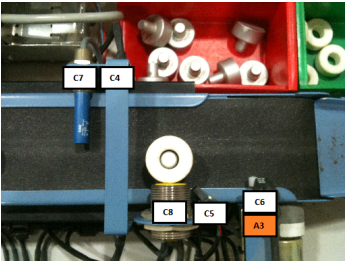
\includegraphics[scale=0.75]{zone.png}
	\captionof{figure}{\textit{zones de contrôle et d'éjection du BCI}}
	\label{fig1}
	\end{center}  

	\paragraph{Travail à réaliser\\}
		Posons les hypothèses suivants:
		\begin{itemize} [label=\ding{70},font=\small \color{black}]
		\item Au maximum une pièce est présente entre les capteurs $C7$ et $C6$.
		\item Le convoyeur à bande $A5$ sera supposé actif à tout instant.
		\end{itemize}
\chapter{\textsc{Analyse et modélisation du procédé}}
%\addcontentsline{toc}{chapter}{\textsc{Analyse et modélisation du prodécé}}

	\section{\textsc{Les dispositions possibles des capteurs $C5$ et $C8$}}	
	\paragraph{} 
	Comme les deux capteurs $C5$ et $C8$ sont de nature physique différente, les zones respectives dans laquelle ils peuvent détecter une pièce ne sont pas identiques. Cependant, la conception de la maquette fait que ces deux zones se chevauchent. La figure suivante représente les quatres dispositions possibles:
	
	\begin{center}
	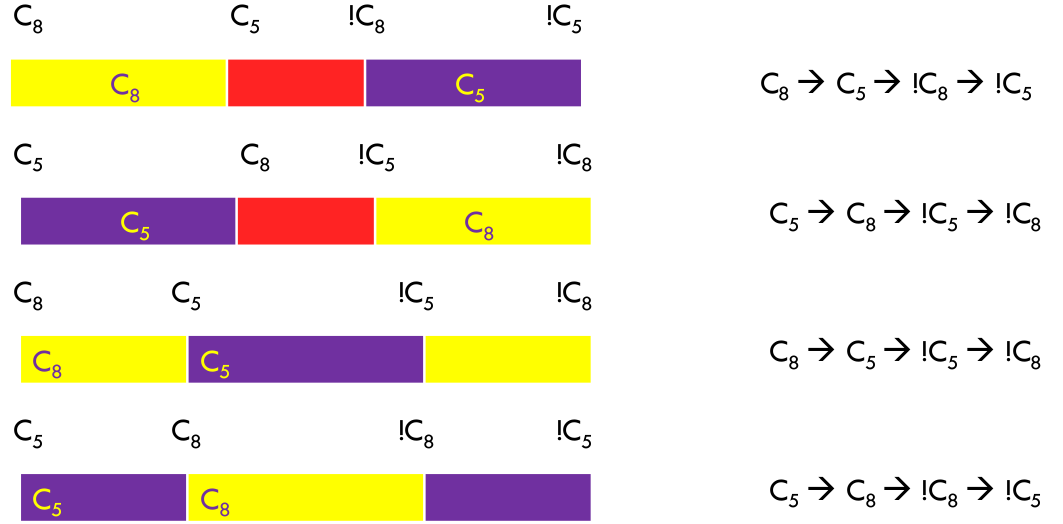
\includegraphics[scale=0.4]{c5.png}
	\captionof{figure}{\textit{Les dispositions possibles des zones de détection des capteurs $C5$ et $C8$}}
	\label{fig2}
	\end{center} 

	\paragraph{} Après avoir fait un test, on constate que c'est la première possibilité qui est réalisée sur la maquette. 
	

	\section{\textsc{Les séquences possibles}}
	
		\paragraph{}
		Considérons à présent les deux hypothèses énoncées plus haut, voici les séquences possibles pour les pièces $bouchon, bouteille \hspace{1mm} et \hspace{1mm}  assemblage$ :
		\paragraph{Bouchon :}
		$C4 \rightarrow \overline{C4} \rightarrow C5 \rightarrow \overline{C5} \rightarrow C6$
		\paragraph{Bouteille :}
		$C7 \rightarrow \overline{C7} \rightarrow C4 \rightarrow \overline{C4} \rightarrow C5 \rightarrow 
		\overline{C5} \rightarrow C6$
		\paragraph{Assemblage :}
		$C7 \rightarrow \overline{C7} \rightarrow C4 \rightarrow \overline{C4} \rightarrow   \textbf{[} ( C5 \rightarrow 
		C8 \rightarrow \overline{C5} \rightarrow \overline{C8}) \vee (C8 \rightarrow 
		C5 \rightarrow \overline{C8} \rightarrow \overline{C5}) \vee (C5 \rightarrow 
		C8 \rightarrow \overline{C8} \rightarrow \overline{C5}) \vee ( C8 \rightarrow 
		C5 \rightarrow \overline{C5} \rightarrow \overline{C8} )\textbf{]} \rightarrow C6$
				
		\section{\textsc{L'expression régulière}}
		
		 On trouve :\\
		 $X0 \rightarrow C7X1 + C7X19 + C4X8 + \varepsilon\\
		 X1 \rightarrow \overline{C7} X2 + \varepsilon\\
		 X2 \rightarrow C4 X3 + \varepsilon\\
		 X3 \rightarrow \overline{C4} X4 + \varepsilon\\
		 X4 \rightarrow C5 X5 + \varepsilon\\
		 X5 \rightarrow \overline{C5} X6 + \varepsilon\\
		 X6 \rightarrow C6 X7 + \varepsilon\\
		 X7 \rightarrow bouteille X13 + \varepsilon\\
		 X13 \rightarrow ADMIS \hspace{1mm} X17 + EJECT \hspace{1mm} X18 + \varepsilon\\
		 X17 \rightarrow \overline{C6} X0 + \varepsilon\\
		 X18 \rightarrow A3 X41 + \varepsilon\\
		 X41 \rightarrow \overline{C6} X42 + \varepsilon\\
		 X42 \rightarrow \overline{A3} X0 + \varepsilon\\\\ $
		 Ou oncore :\\
		 $X8 \rightarrow \overline{C4} X9 + \varepsilon\\
		 X9 \rightarrow C5 X10 + \varepsilon\\
		 X10 \rightarrow \overline{C5} X11 + \varepsilon\\
		 X11 \rightarrow C6 X12 + \varepsilon\\
		 X12 \rightarrow bouchon X14 + \varepsilon\\
		 X14 \rightarrow ADMIS \hspace{1mm} X15 + EJECT \hspace{1mm} X16 + \varepsilon\\
		 X15 \rightarrow \overline{C6} X0 + \varepsilon\\
		 X16 \rightarrow A3 X39 + \varepsilon\\
		 X39 \rightarrow \overline{C6} X40 + \varepsilon\\
		 X40 \rightarrow \overline{A3} X0 + \varepsilon\\\\ $
		 Mais aussi : \\
		 $X19 \rightarrow \overline{C7} X20 + \varepsilon\\
		 X20 \rightarrow C4 X21 + \varepsilon\\
		 X21 \rightarrow \overline{C4} X22 + \varepsilon\\
		 X22 \rightarrow C5 X23 + C8 X24 + \varepsilon\\
		 X23 \rightarrow C8 X25 + \varepsilon\\
		 X25 \rightarrow \overline{C5} X27 + \overline{C8} X28 + \varepsilon\\
		 X27 \rightarrow \overline{C8} X32 + \varepsilon\\
		 X28 \rightarrow \overline{C5} X31 + \varepsilon\\
		 X31 \rightarrow C6 X35 + \varepsilon\\
		 X32 \rightarrow C6 X35 + \varepsilon\\
		 X24 \rightarrow C5 X26 + \varepsilon\\
		 X26 \rightarrow \overline{C5} X29 + \overline{C8} X30 + \varepsilon\\
		 X29 \rightarrow \overline{C8} X33 + \varepsilon\\
		 X30 \rightarrow \overline{C5} X34 + \varepsilon\\
		 X33 \rightarrow C6 X35 + \varepsilon\\
		 X34 \rightarrow C6 X35 + \varepsilon\\
		 X35 \rightarrow assemblage X36 + \varepsilon\\
		 X36 \rightarrow ADMIS \hspace{1mm} X37 + EJECT \hspace{1mm} X38 + \varepsilon\\
		 X37 \rightarrow \overline{C6} X0 + \varepsilon\\
		 X38 \rightarrow A3 X43 + \varepsilon\\
		 X43 \rightarrow \overline{C6} X44 + \varepsilon\\
		 X44 \rightarrow \overline{A3} X0 + \varepsilon\\\\ $
		 Après réduction on trouve : \\[0.25 cm]
		 
		  
		 $X1 \rightarrow C7 \overline{C7}  C4 \overline{C4} C5 \overline{C5} C6 bouteille( ADMIS \hspace{1mm} \overline{C6} + EJECT \hspace{1mm} A3 \overline{C6} \overline{A3} ) X0\\ 		 
		 + C7 \overline{C7} C4 \overline{C4} C5 \overline{C5} C6 bouteille ( EJECT \hspace{1mm} A3 \overline{C6} + EJECT \hspace{1mm} A3 + ADMIS \hspace{1mm} + EJECT \hspace{1mm} ) + C7 \overline{C7} C4 \overline{C4} C5 \overline{C5} C6 bouteille + C7 \overline{C7} C4 \overline{C4} C5 \overline{C5} C6 + C7 \overline{C7} C4 \overline{C4} C5 \overline{C5} \\+ C7 \overline{C7} C4 \overline{C4} C5 + C7 \overline{C7} C4 \overline{C4} + C7 \overline{C7} C4 + C7 \overline{C7} + C7 + \varepsilon \\\\ $
		 
		 
		 
		 $X8 \rightarrow  C4 \overline{C4} C5 \overline{C5} C6 bouchon ( ADMIS \hspace{1mm} \overline{C6} + EJECT A3 \overline {C6A3} )X0 \\		 
		 + C4 \overline{C4} C5 \overline{C5} C6 bouchon EJECT \hspace{1mm} A3 \overline{C6} + C4 \overline{C4} C5 \overline{C5} C6 bouchon EJECT \hspace{1mm} A3\\ + C4 \overline{C4} C5 \overline{C5} C6 bouchon EJECT \hspace{1mm} + C4 \overline{C4} C5 \overline{C5} C6 bouchon ADMIS \hspace{1mm}\\ + C4 \overline{C4} C5 \overline{C5} C6 bouchon + C4 \overline{C4} C5 \overline{C5} C6 + C4 \overline{C4} C5 \overline{C5} + C4 \overline{C4} C5 + C4 \overline{C4} + C4 + \varepsilon \\\\ $
		 
		 
		 $X19 \rightarrow C7\overline{C7} C4 \overline{C4} [C8C5 ( \overline{C5} \overline{C8} C6 assemblage ( ADMIS \hspace{1mm} \overline{C6} + EJECT \hspace{1mm} A3 \overline{C6A3} ) \\+ \overline{C8} \overline{C8} C6 assemblage ( ADMIS \hspace{1mm} \overline{C6} + EJECT \hspace{1mm} A3 \overline{C6A3} ) ) \\+ C5C8 ( \overline{C8} \overline{C5} C6 assemblage ( ADMIS \hspace{1mm} \overline{C6} + EJECT \hspace{1mm} A3 \overline{C6A3} ) \\+ \overline{C5} \overline{C8} C6 assemblage ( ADMIS \hspace{1mm} \overline{C6} + EJECT \hspace{1mm} A3 \overline{C6A3} ) ) ]
		  X0 	 + C7\overline{C7}  C4 \overline{C4} C8 C5 ( \overline{C5} + \overline{C8} ) \overline{C8}  C6 assemblage\\ (   EJECT \hspace{1mm}A3 \overline{C6} + EJECT \hspace{1mm} A3 + EJECT \hspace{1mm} + ADMIS ) + C7 \overline{C7}  C4 \overline{C4} C8C5 ( \overline{C5} + \overline{C8} ) \overline{C8} C6 assemblage + C7 \overline{C7}  C4 \overline{C4} C8C5 ( \overline{C5} + \overline{C8} ) \overline{C8} C6 + C7 \overline{C7}  C4 \overline{C4} C8C5 ( \overline{C5} + \overline{C8} ) \overline{C8}  + C7 \overline{C7}  C4 \overline{C4} C8C5 \overline{C5} + C7 \overline{C7}  C4 \overline{C4} C8C5 \overline{C8} + C7 \overline{C7}  C4 \overline{C4} C8C5 + C7 \overline{C7}  C4 \overline{C4} C8 + C7 \overline{C7}  C4 \overline{C4} C5 C8 \overline{C8} \overline{C5} C6 assemblage ( EJECT \hspace{1mm}A3 \overline{C6} + EJECT \hspace{1mm} A3 + EJECT \hspace{1mm} + ADMIS ) + C7 \overline{C7}  C4 \overline{C4} C5C8 \overline{C5} \overline{C8} C6 assemblage ( EJECT \hspace{1mm}A3 \overline{C6} + EJECT \hspace{1mm} A3 + EJECT \hspace{1mm} + ADMIS ) + C7 \overline{C7}  C4 \overline{C4} C5C8 \overline{C8} \overline{C5} C6 assemblage \\+ C7 \overline{C7}  C4 \overline{C4} C5C8 \overline{C5} \overline{C8} C6 assemblage + C7 \overline{C7}  C4 \overline{C4} C5C8  \overline{C8} \overline{C5} C6 \\+ C7 \overline{C7}  C4 \overline{C4} C5C8  \overline{C5} \overline{C8} C6 + C7 \overline{C7}  C4 \overline{C4} C5 C8  \overline{C8} \overline{C5} + C7 \overline{C7}  C4 \overline{C4} C5C8  \overline{C5} \overline{C8} + C7 \overline{C7}  C4 \overline{C4} C5C8  \overline{C8} + C7 \overline{C7}  C4 \overline{C4} C5C8  \overline{C5} + C7 \overline{C7}  C4 \overline{C4} C5C8 + C7 \overline{C7}  C4 \overline{C4} C5 + \overline{C7}  C4 \overline{C4} + C7 \overline{C7}  C4 + C7 \overline{C7}  + C7 + \varepsilon\\\\ $ 
		 
		 
		 Enfin l'expression régulière correspondante s'écrit comme suit : \\

$ER =   \textbf{(} C7 \overline{C7}  C4 \overline{C4} C5 \overline{C5} C6 bouteille( ADMIS \hspace{1mm} \overline{C6} + EJECT \hspace{1mm} A3 \overline{C6} \overline{A3} ) \\+ C7\overline{C7} C4 \overline{C4} [C8C5 ( \overline{C5} \overline{C8} C6 assemblage ( ADMIS \hspace{1mm} \overline{C6} + EJECT \hspace{1mm} A3 \overline{C6A3} ) + \overline{C8} \overline{C8} C6 assemblage ( ADMIS \hspace{1mm} \overline{C6} + EJECT \hspace{1mm} A3 \overline{C6A3} ) ) \\+ C5C8 ( \overline{C8} \overline{C5} C6 assemblage ( ADMIS \hspace{1mm} \overline{C6} + EJECT \hspace{1mm} A3 \overline{C6A3} ) \\+ \overline{C5} \overline{C8} C6 assemblage ( ADMIS \hspace{1mm} \overline{C6} + EJECT \hspace{1mm} A3 \overline{C6A3} ) ) ] \\+ C4 \overline{C4} C5 \overline{C5} C6 bouchon ( ADMIS \hspace{1mm} \overline{C6} + EJECT A3 \overline {C6A3} ) \textbf{)}\textbf{*} \\\\ $
$\textbf{(}C7 \overline{C7} C4 \overline{C4} C5 \overline{C5} C6 bouteille ( EJECT \hspace{1mm} A3 \overline{C6} + EJECT \hspace{1mm} A3 + ADMIS \hspace{1mm} + EJECT \hspace{1mm} ) + C7 \overline{C7} C4 \overline{C4} C5 \overline{C5} C6 bouteille  \\+ C7 \overline{C7} C4 \overline{C4} C5 \overline{C5} C6 + C7 \overline{C7} C4 \overline{C4} C5 \overline{C5} + C7 \overline{C7} C4 \overline{C4} C5 + C7 \overline{C7} C4 \overline{C4} + C7 \overline{C7} C4 + C7 \overline{C7} + C7 \\+ 
 C4 \overline{C4} C5 \overline{C5} C6 bouchon EJECT \hspace{1mm} A3 \overline{C6} + C4 \overline{C4} C5 \overline{C5} C6 bouchon EJECT \hspace{1mm} A3\\ + C4 \overline{C4} C5 \overline{C5} C6 bouchon EJECT \hspace{1mm} + C4 \overline{C4} C5 \overline{C5} C6 bouchon ADMIS \hspace{1mm}\\ + C4 \overline{C4} C5 \overline{C5} C6 bouchon + C4 \overline{C4} C5 \overline{C5} C6 + C4 \overline{C4} C5 \overline{C5} + C4 \overline{C4} C5 + C4 \overline{C4} + C4 \\+
   C7\overline{C7}  C4 \overline{C4} C8 C5 ( \overline{C5} + \overline{C8} ) \overline{C8}  C6 assemblage\\ (   EJECT \hspace{1mm}A3 \overline{C6} + EJECT \hspace{1mm} A3 + EJECT \hspace{1mm} + ADMIS ) + C7 \overline{C7}  C4 \overline{C4} C8C5 ( \overline{C5} + \overline{C8} ) \overline{C8} C6 assemblage + C7 \overline{C7}  C4 \overline{C4} C8C5 ( \overline{C5} + \overline{C8} ) \overline{C8} C6 + C7 \overline{C7}  C4 \overline{C4} C8C5 ( \overline{C5} + \overline{C8} ) \overline{C8}  + C7 \overline{C7}  C4 \overline{C4} C8C5 \overline{C5} + C7 \overline{C7}  C4 \overline{C4} C8C5 \overline{C8} + C7 \overline{C7}  C4 \overline{C4} C8C5 + C7 \overline{C7}  C4 \overline{C4} C8 + C7 \overline{C7}  C4 \overline{C4} C5 C8 \overline{C8} \overline{C5} C6 assemblage ( EJECT \hspace{1mm}A3 \overline{C6} + EJECT \hspace{1mm} A3 + EJECT \hspace{1mm} + ADMIS ) + C7 \overline{C7}  C4 \overline{C4} C5C8 \overline{C5} \overline{C8} C6 assemblage ( EJECT \hspace{1mm}A3 \overline{C6} + EJECT \hspace{1mm} A3 + EJECT \hspace{1mm} + ADMIS ) + C7 \overline{C7}  C4 \overline{C4} C5C8 \overline{C8} \overline{C5} C6 assemblage \\+ C7 \overline{C7}  C4 \overline{C4} C5C8 \overline{C5} \overline{C8} C6 assemblage + C7 \overline{C7}  C4 \overline{C4} C5C8  \overline{C8} \overline{C5} C6 \\+ C7 \overline{C7}  C4 \overline{C4} C5C8  \overline{C5} \overline{C8} C6 + C7 \overline{C7}  C4 \overline{C4} C5 C8  \overline{C8} \overline{C5} + C7 \overline{C7}  C4 \overline{C4} C5C8  \overline{C5} \overline{C8} + C7 \overline{C7}  C4 \overline{C4} C5C8  \overline{C8} + C7 \overline{C7}  C4 \overline{C4} C5C8  \overline{C5} + C7 \overline{C7}  C4 \overline{C4} C5C8 + C7 \overline{C7}  C4 \overline{C4} C5 + \overline{C7}  C4 \overline{C4} + C7 \overline{C7}  C4 + C7 \overline{C7}  + C7 + \varepsilon \textbf{)} \\\\ $
   
  \pagebreak
		 \section{\textsc{Graphe de l'automate (Procédé)}} 
		 
		 	\begin{center}
			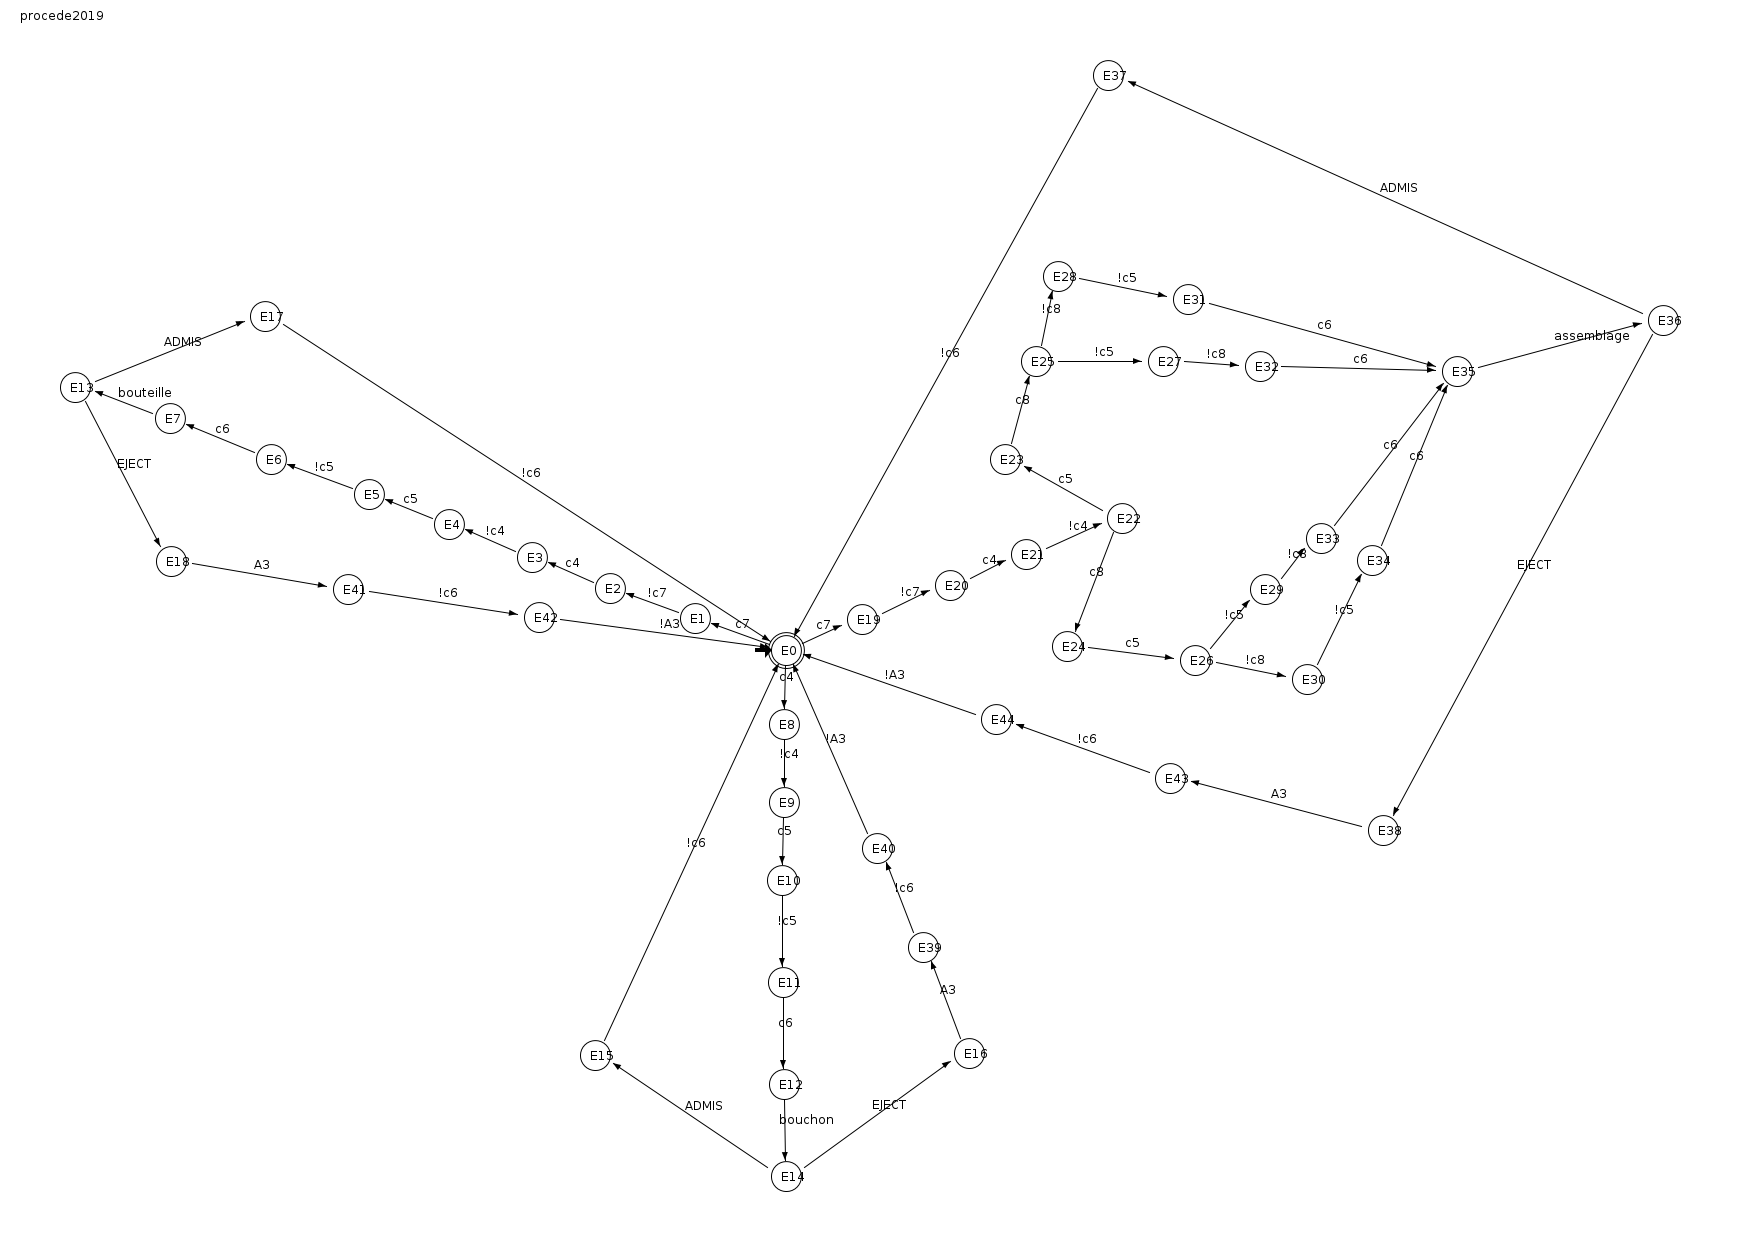
\includegraphics[scale=0.25]{procede.png}
			\captionof{figure}{\textit{Le procédé modélisé sous SEDMA}}
			\label{fig3}
			\end{center} 
			\paragraph{Remarque :} Pour plus de clarté nous vous conseillons de bien vouloir zoomer sur l'image ou bien de cliquer sur \href{https://github.com/kherbicheali/SED\_report/tree/master/BCI\_SEDMA/}{ce lien github}  contenant notre travail ainsi que tous les graphes faits sous SEDMA. 
	
			\section{\textsc{Premier langage marqué reconnu par l'automate}}
			
			Pour des états finaux correspondant à l’éjection ou l’admission d’une pièce reconnue (bouchon, bouteille ou assemblage) et un état initial correspondant à un tapis vide, on trouve :\\
		 $X0 \rightarrow C7X1 + C7X19 + C4X8 \\
		 X1 \rightarrow \overline{C7} X2\\
		 X2 \rightarrow C4 X3\\
		 X3 \rightarrow \overline{C4} X4\\
		 X4 \rightarrow C5 X5\\
		 X5 \rightarrow \overline{C5} X6\\
		 X6 \rightarrow C6 X7\\
		 X7 \rightarrow bouteille X13\\
		 X13 \rightarrow ADMIS \hspace{1mm} X17 + EJECT \hspace{1mm} X18\\
		 X17 \rightarrow  \varepsilon\\
		 X18 \rightarrow \varepsilon\\
		 X41 \rightarrow \overline{C6} X42\\
		 X42 \rightarrow \overline{A3} X0\\\\ $
		 Ou oncore :\\
		 $X8 \rightarrow \overline{C4} X9\\
		 X9 \rightarrow C5 X10\\
		 X10 \rightarrow \overline{C5} X11\\
		 X11 \rightarrow C6 X12\\
		 X12 \rightarrow bouchon X14 + \varepsilon\\
		 X14 \rightarrow ADMIS \hspace{1mm} X15 + EJECT \hspace{1mm} X16\\
		 X15 \rightarrow \varepsilon\\
		 X16 \rightarrow \varepsilon\\
		 X39 \rightarrow \overline{C6} X40\\
		 X40 \rightarrow \overline{A3} X0\\\\ $
		 Mais aussi : \\
		 $X19 \rightarrow \overline{C7} X20\\
		 X20 \rightarrow C4 X21\\
		 X21 \rightarrow \overline{C4} X22\\
		 X22 \rightarrow C5 X23 + C8 X24 \\
		 X23 \rightarrow C8 X25\\
		 X25 \rightarrow \overline{C5} X27 + \overline{C8} X28\\
		 X27 \rightarrow \overline{C8} X32\\
		 X28 \rightarrow \overline{C5} X31\\
		 X31 \rightarrow C6 X35\\
		 X32 \rightarrow C6 X35\\
		 X24 \rightarrow C5 X26\\
		 X26 \rightarrow \overline{C5} X29 + \overline{C8} X30\\
		 X29 \rightarrow \overline{C8} X33\\
		 X30 \rightarrow \overline{C5} X34\\
		 X33 \rightarrow C6 X35\\
		 X34 \rightarrow C6 X35\\
		 X35 \rightarrow assemblage X36\\
		 X36 \rightarrow ADMIS \hspace{1mm} X37 + EJECT \hspace{1mm} X38\\
		 X37 \rightarrow \varepsilon\\
		 X38 \rightarrow \varepsilon\\
		 X43 \rightarrow \overline{C6} X44\\
		 X44 \rightarrow \overline{A3} X0\\\\ $
		 
		 Après réduction on trouve : \\[0.25 cm]
		 $X1 \rightarrow  \overline{C7} C4 \overline{C4} C5 \overline{C5} C6 bouteille EJECT \hspace{1mm} A3 \overline{C6A3} X0 + \overline{C7} C4 \overline{C4} C5 \overline{C5} C6 bouteilleADMIS\\\\ $
		
		 %$X8 \rightarrow \overline{C7} X2$
		 
		 Enfin l'expression régulière du langage marqué reconnu par l'automate s'écrit comme suit : \\
		 
		 
		 
		% \pagebreak 
		 \section{\textsc{Second langage marqué reconnu par l'automate}}
   		 
		 Pour des états finaux correspondant uniquement à l’admission d’une pièce reconnue (bouchon, bouteille ou assemblage) et un état initial correspondant à un tapis vide, on trouve :\\
		 
		 $X0 \rightarrow C7X1 + C7X19 + C4X8\\
		 X1 \rightarrow \overline{C7} X2\\
		 X2 \rightarrow C4 X3\\
		 X3 \rightarrow \overline{C4} X4\\
		 X4 \rightarrow C5 X5\\
		 X5 \rightarrow \overline{C5} X6\\
		 X6 \rightarrow C6 X7\\
		 X7 \rightarrow bouteille X13\\
		 X13 \rightarrow ADMIS \hspace{1mm} X17 + EJECT \hspace{1mm} X18\\
		 X17 \rightarrow \varepsilon\\
		 X18 \rightarrow A3 X41\\
		 X41 \rightarrow \overline{C6} X42\\
		 X42 \rightarrow \overline{A3} X0\\\\ $
		 Ou oncore :\\
		 $X8 \rightarrow \overline{C4} X9\\
		 X9 \rightarrow C5 X10\\
		 X10 \rightarrow \overline{C5} X11\\
		 X11 \rightarrow C6 X12\\
		 X12 \rightarrow bouchon X14\\
		 X14 \rightarrow ADMIS \hspace{1mm} X15 + EJECT \hspace{1mm} X16\\
		 X15 \rightarrow \varepsilon\\
		 X16 \rightarrow A3 X39\\
		 X39 \rightarrow \overline{C6} X40\\
		 X40 \rightarrow \overline{A3} X0\\\\ $
		 Mais aussi : \\
		 $X19 \rightarrow \overline{C7} X20\\
		 X20 \rightarrow C4 X21\\
		 X21 \rightarrow \overline{C4} X22\\
		 X22 \rightarrow C5 X23 + C8 X24\\
		 X23 \rightarrow C8 X25\\
		 X25 \rightarrow \overline{C5} X27 + \overline{C8} X28\\
		 X27 \rightarrow \overline{C8} X32\\
		 X28 \rightarrow \overline{C5} X31\\
		 X31 \rightarrow C6 X35\\
		 X32 \rightarrow C6 X35\\
		 X24 \rightarrow C5 X26\\
		 X26 \rightarrow \overline{C5} X29 + \overline{C8} X30\\
		 X29 \rightarrow \overline{C8} X33\\
		 X30 \rightarrow \overline{C5} X34\\
		 X33 \rightarrow C6 X35\\
		 X34 \rightarrow C6 X35\\
		 X35 \rightarrow assemblage X36\\
		 X36 \rightarrow ADMIS \hspace{1mm} X37 + EJECT \hspace{1mm} X38\\
		 X37 \rightarrow \varepsilon\\
		 X38 \rightarrow A3 X43\\
		 X43 \rightarrow \overline{C6} X44\\
		 X44 \rightarrow \overline{A3} X0\\\\ $
   				
		Enfin l'expression régulière du langage marqué reconnu par l'automate s'écrit comme suit : \\		
		
	 \pagebreak

\chapter{\textsc{Modélisation des objectifs}} 
%\addcontentsline{toc}{chapter}{\textsc{Modélisation des objectifs}}					 
		 
		 \section{\textsc{Premier cahier des charges}} 
		 
		 	\begin{center}
			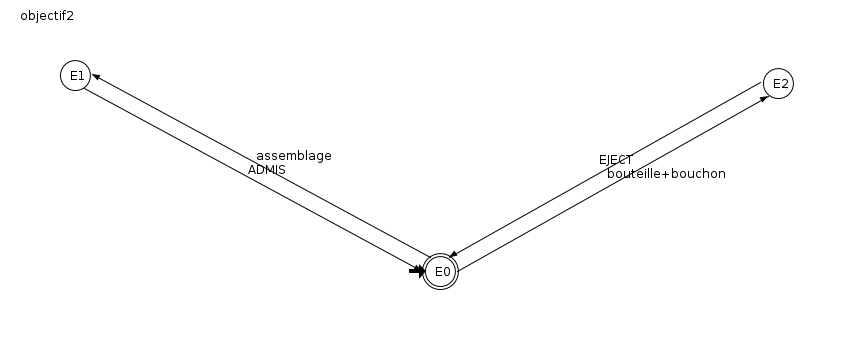
\includegraphics[scale=0.4]{obj1.png}
			\captionof{figure}{\textit{Le premier objectif modélisé sous SEDMA}}
			\label{fig4}
			\end{center} 
		
		 \section{\textsc{Second cahier des charges}} 
		 
		 	\begin{center}
			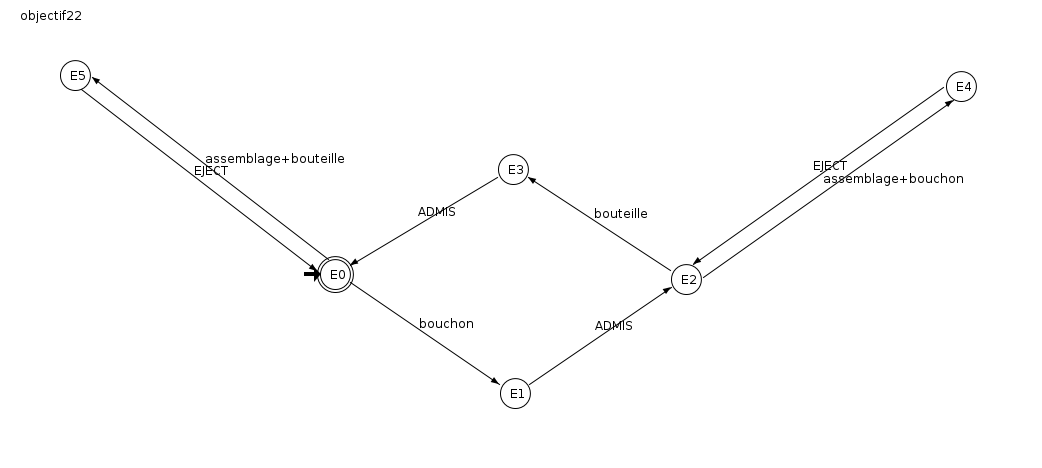
\includegraphics[scale=0.4]{obj2.png}
			\captionof{figure}{\textit{Le second objectif modélisé sous SEDMA}}
			\label{fig5}
			\end{center} 
			
	 \pagebreak

\chapter{\textsc{Le produit parallèle des deux modèles}}

		  \section{\textsc{La première commande}}
		    
		  \begin{center}
			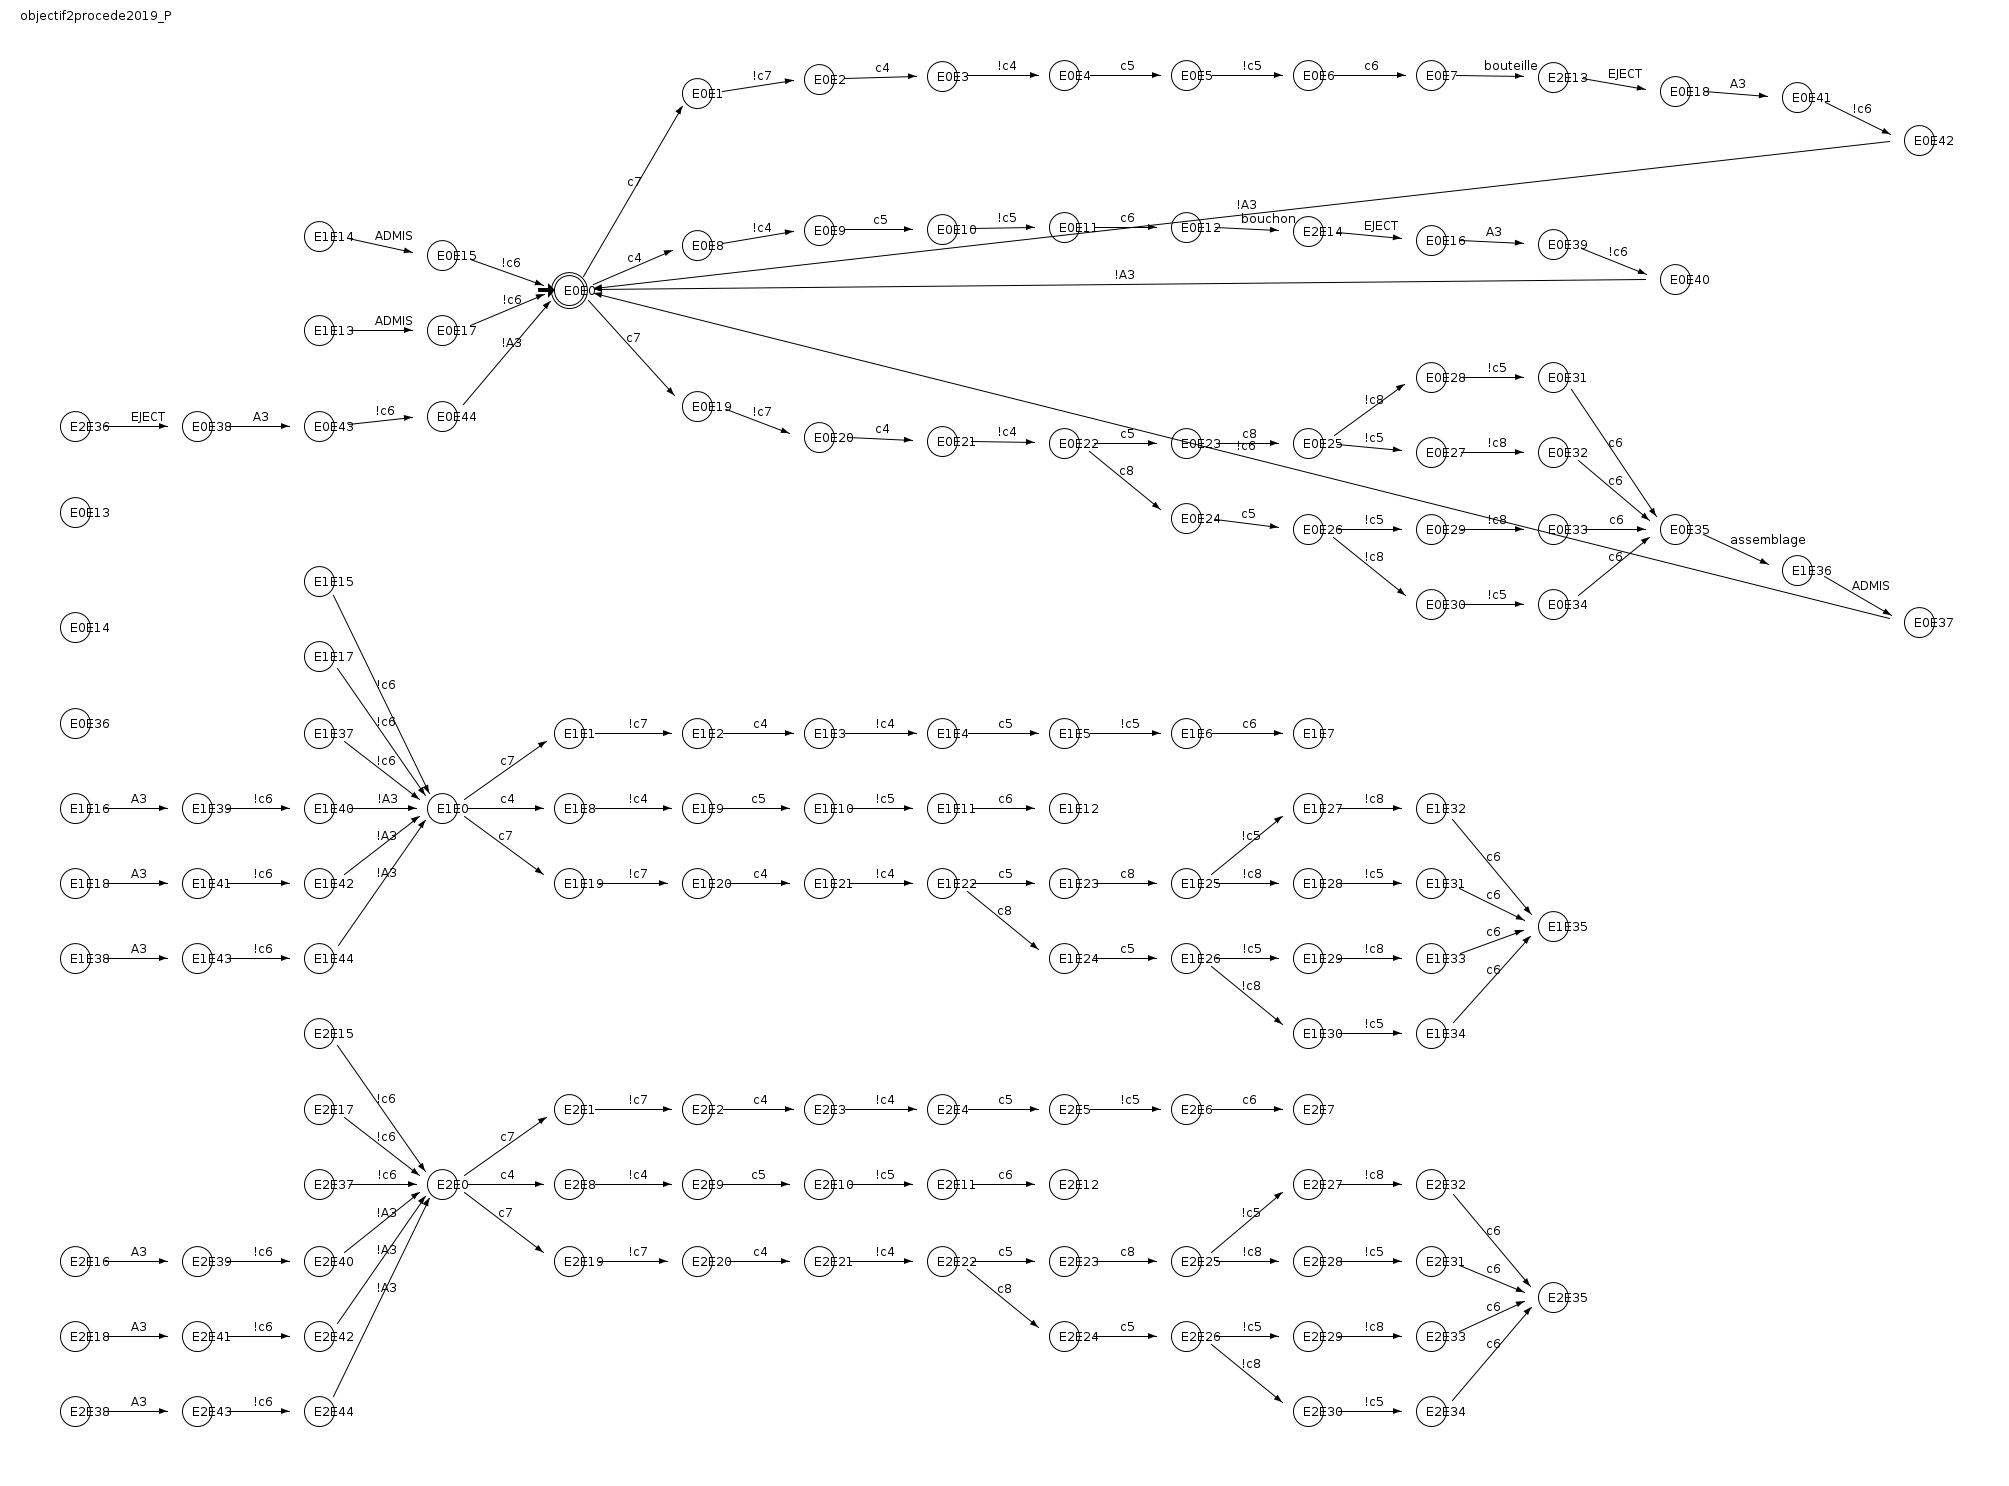
\includegraphics[scale=0.2]{com1.png}
			\captionof{figure}{\textit{La première commande non simplifiée modélisée sous SEDMA}}
			\label{fig6}
			\end{center}		    
		    
		  \section{\textsc{La seconde commande}}
			
			\begin{center}
			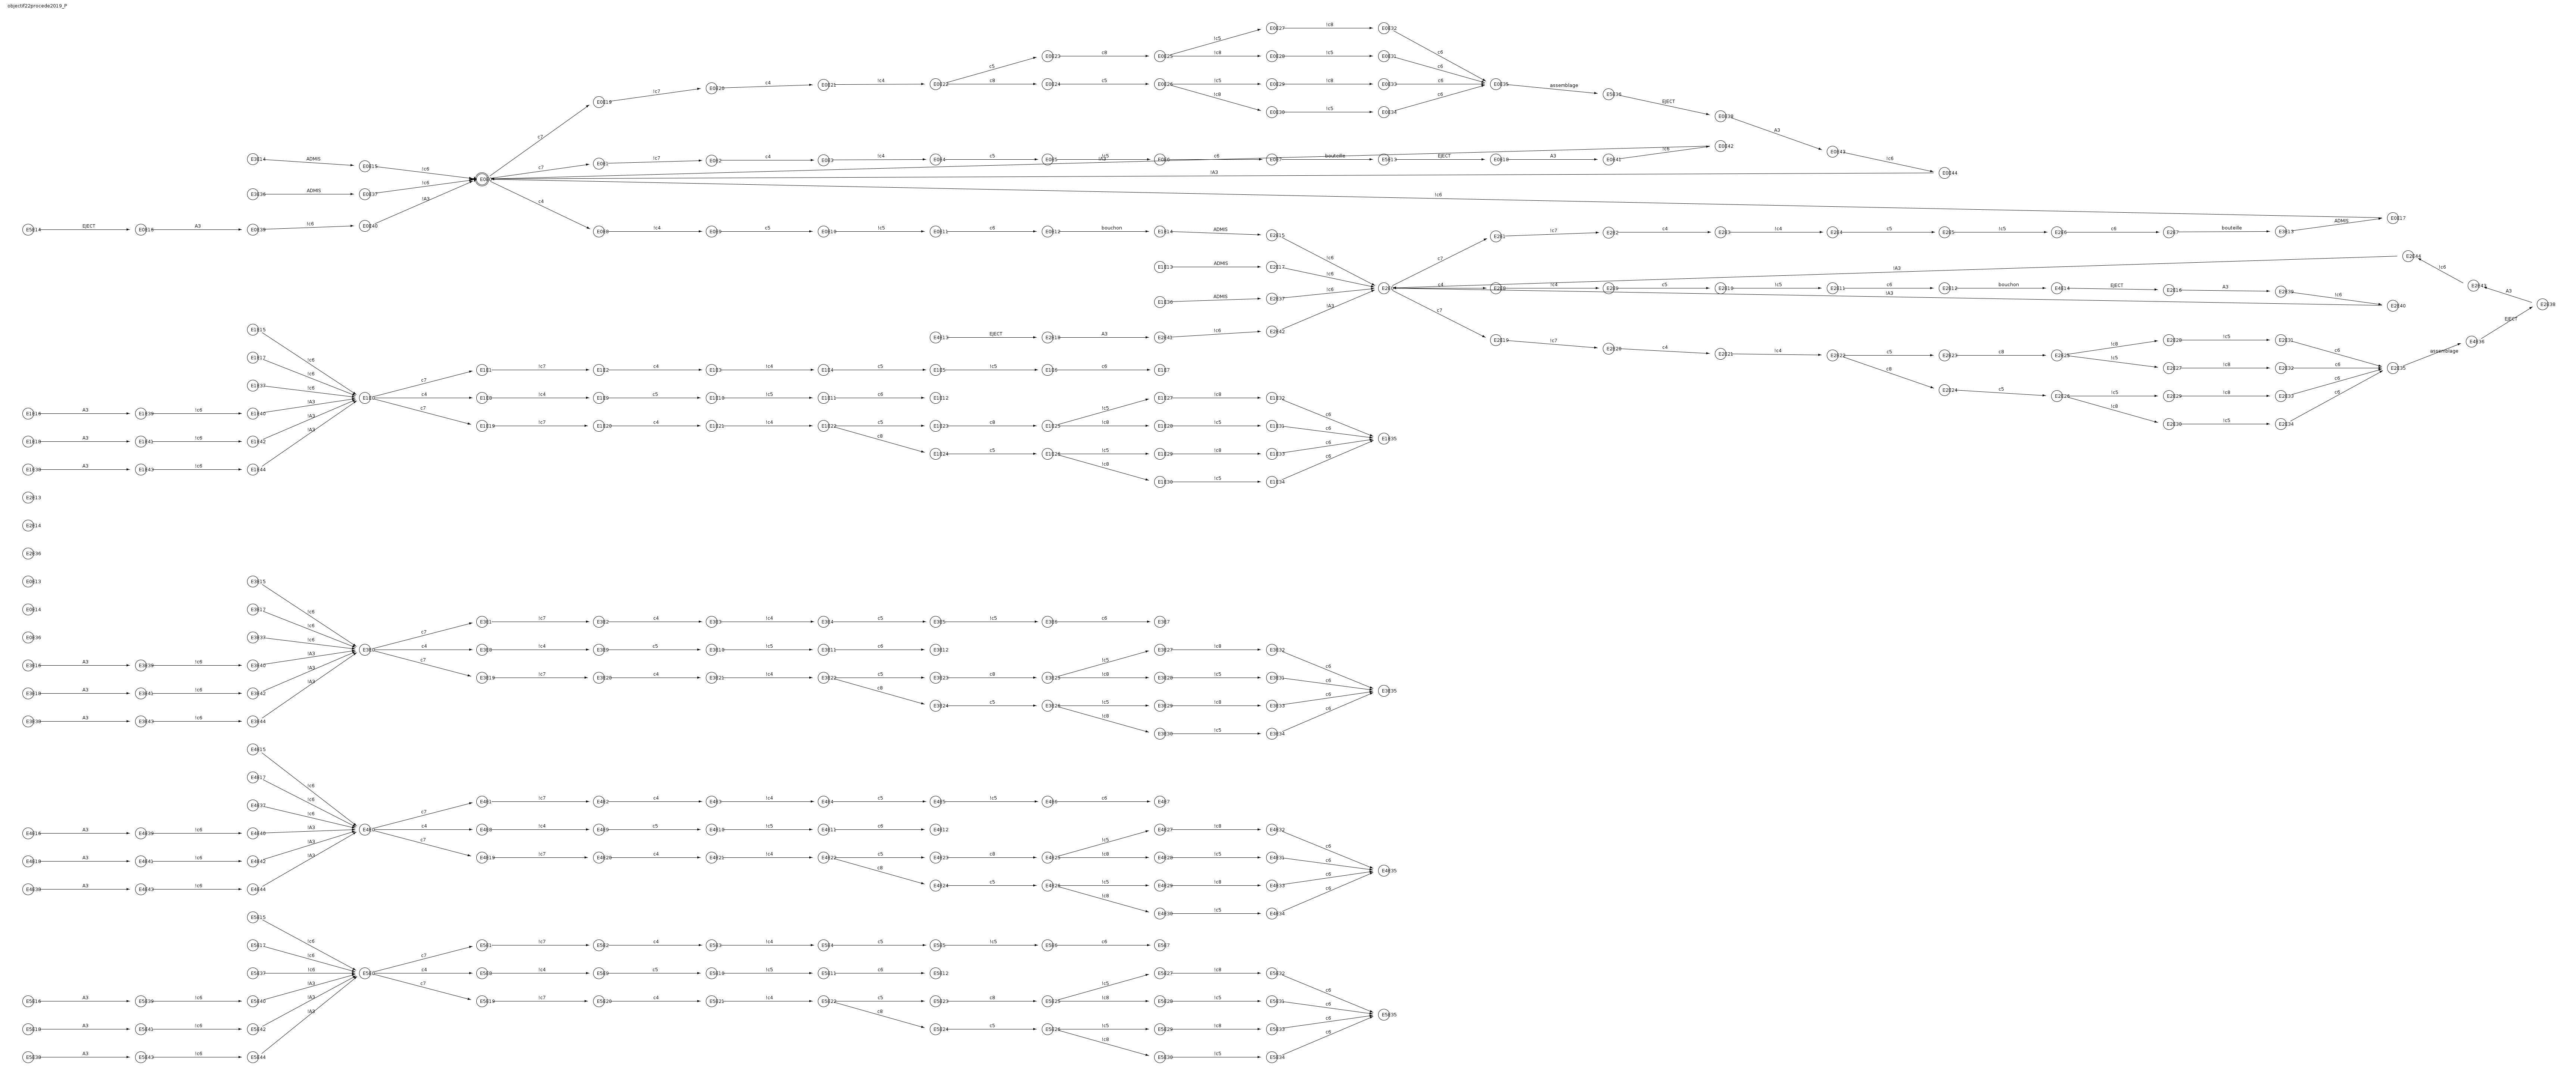
\includegraphics[scale=0.07]{com2.png}
			\captionof{figure}{\textit{La seconde commande non simplifiée modélisée sous SEDMA}}
			\label{fig7}
			\end{center}		  
		  
		   \pagebreak
		 \chapter{\textsc{Simplification des commandes}}
		 
		 \par Afin de simplifier les commandes, on doit passer par un $TRIM$ pour ne garder que les états accessibles et les états co-accessibles, il faut aussi transformer la commande en $automate \hspace{1mm} de \hspace{1mm} Moore$ pour que la sortie puisse dépendre de l'état en cours.\\
		  
		 
		  \section{\textsc{La première commande simplifiée}}
		  
		    \begin{center}
			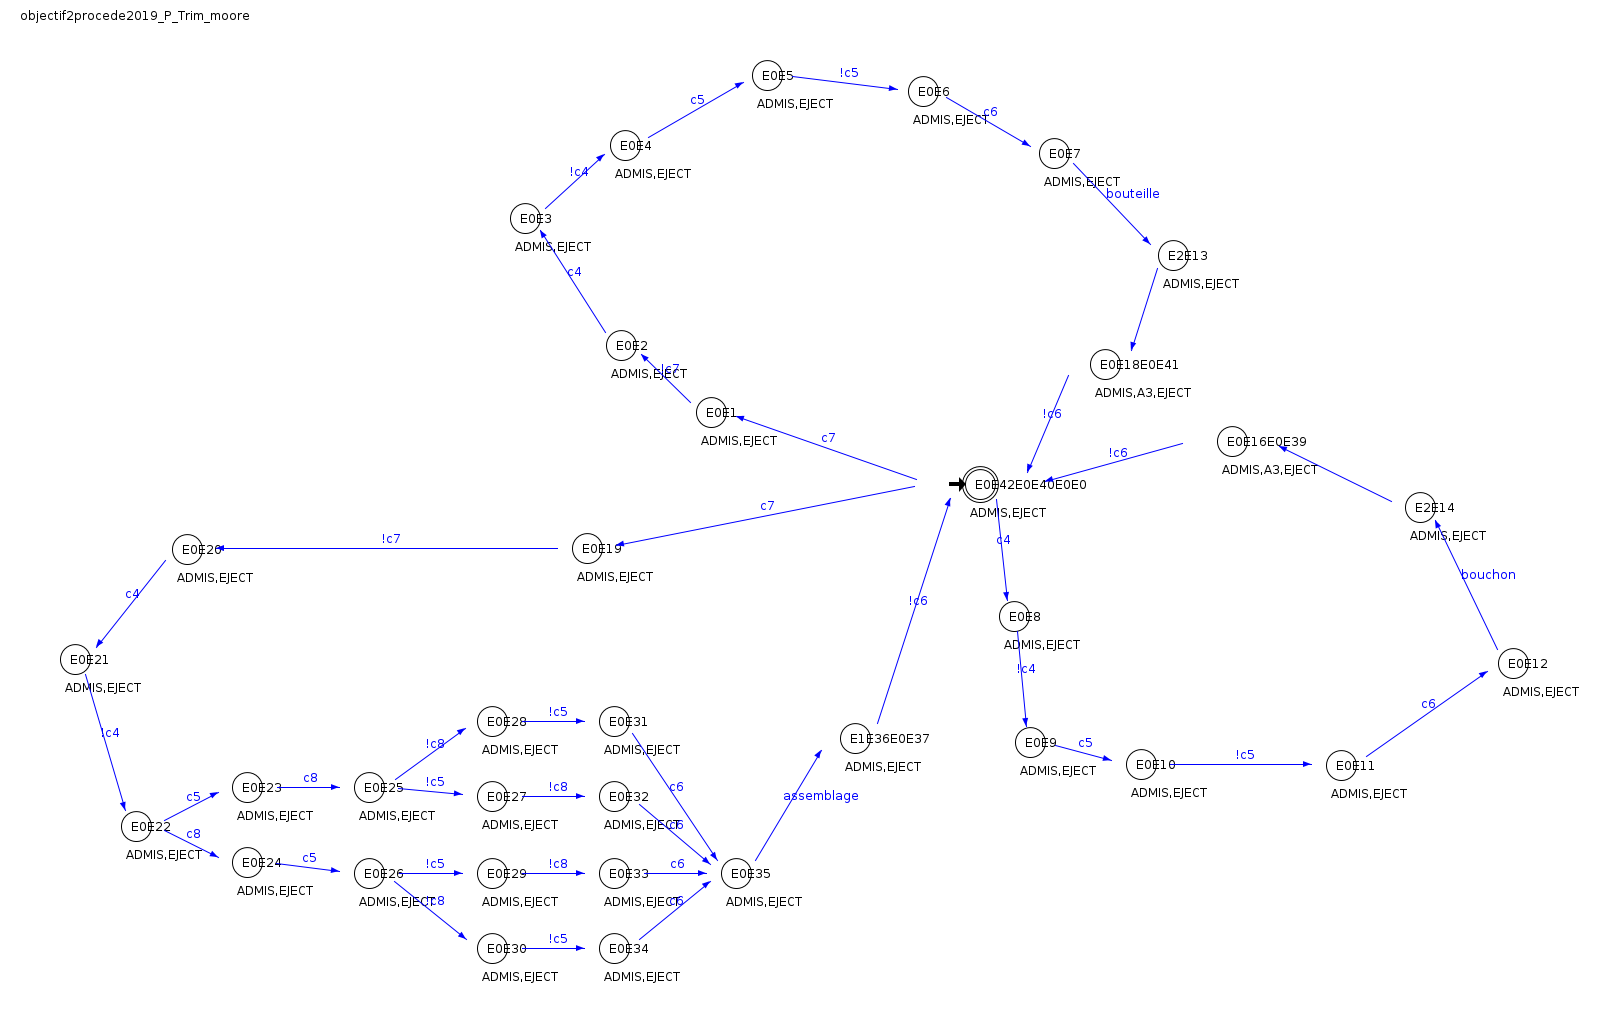
\includegraphics[scale=0.275]{com1s.png}
			\captionof{figure}{\textit{La première commande simplifiée modélisée sous SEDMA}}
			\label{fig8}
			\end{center}	
			
		  \section{\textsc{La seconde commande simplifiée}}
			
			\begin{center}
			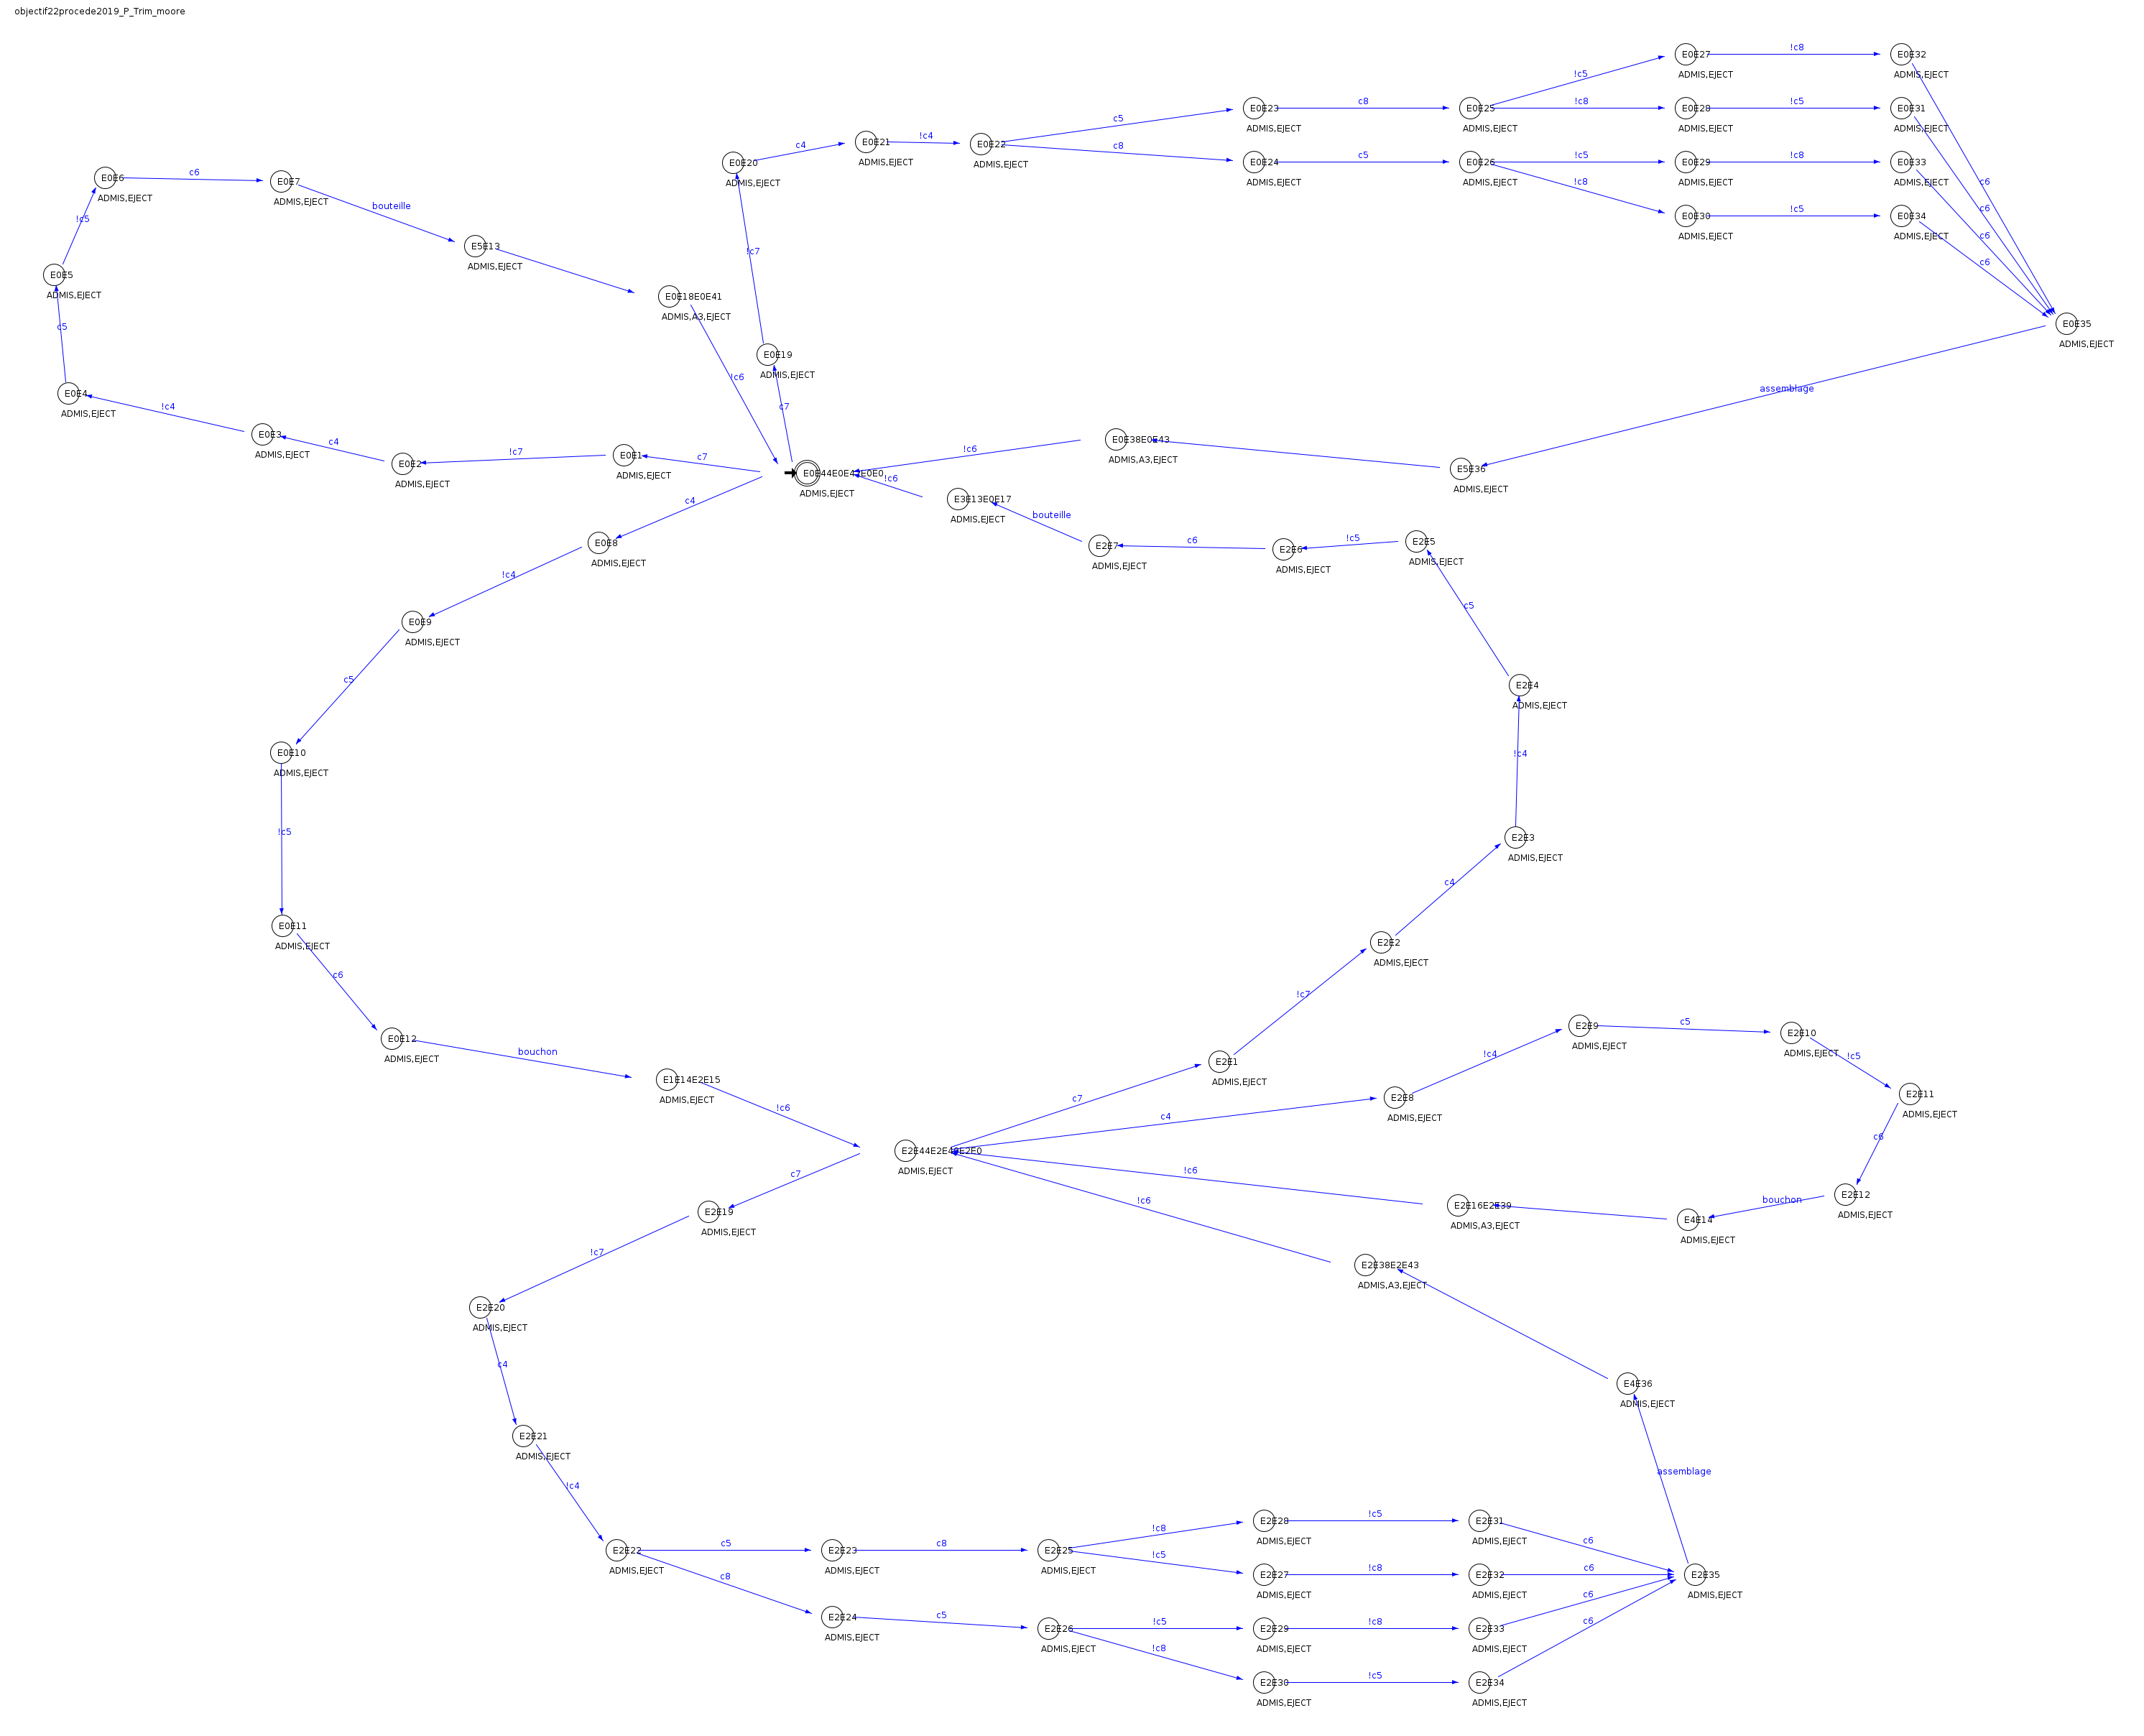
\includegraphics[scale=0.15]{com2s.png}
			\captionof{figure}{\textit{La seconde commande simplifiée modélisée sous SEDMA}}
			\label{fig9}
			\end{center}	
		 
\chapter*{\textsc{Conclusion}}
\addcontentsline{toc}{chapter}{\textsc{Conclusion}}
 
 \paragraph{} Cette séance de travaux pratiques nous a initié au logicieLs SEDMA et UNITY et durant ces quatre heure nous avons concrétisé l'étude théorique faite en cours et en travaux dirigés comme contruire un modèle du procédé à base du cahier des charges, définir un objectif et enfin déduire une commande puis la simplifier dans le but  d'extraire son code ST de SEDMA et l'injecter dans UNITY pour ensuite faire marcher la maquette.    
%\input{chap2.tex}
%\input{chap4&5.tex}
%\input{conclusion.tex}
%\input{annexes.tex}
%*********************** Bibliographie ************ 
\bibliographystyle{alpha}
\bibliography{biblio}  



\end{document}